\section{Approach to Discover the Case Perspective}
\label{sec:bpm2017approach}

%In this section, we describe our approach for mining software development projects. First, we give an overview of the approach itself, then we formally define concepts required by our technique.

%Version control systems (VCSs) are used in projects to ensure reliable collaboration.
%We build our technique on \gls{vcs}. In this context, project participants work on files (e.g., text, source code, spread sheets) and commit their changes to a central repository, which maintains information on the work history.

We propose a technique to extract and represent the work history and the dependencies among artifacts of a project-oriented business process. The technique takes as input a \gls{vcs} log and produces analysis data that describe the evolution of the artifacts, along with metrics about their distance and their similarity in terms of work.
The process is depicted in \Cref{fig:visualization-process} and consists of three successive steps towards extracting hidden work dependencies from \gls{vcs} event data. The method works under three main assumptions. First, we assume a \emph{meaningful tree structure}, i.e. the project participants organize the files in a representative hierarchy (e.g., spatially separating documentation from testing into different folders). Second, project participants perform \emph{regular commits} in the \gls{vcs}. Third, project participants write \emph{descriptive comments} that allow other members to understand the changes.

%\begin{itemize}
%	\item [A1:] {\bf Meaningful file tree structure.} The file tree structure in a project represents the structure of work of the project participants.
%	\item [A2:] {\bf Frequent commits.} Commits to the VCS are regularly performed.
%	\item [A3:] {\bf Meaningful comments.} The comments included by project participant when committing their work represent the changes done to the file being commit.
%\end{itemize}
%\vspace*{-.5cm}
\begin{figure}[h]
	\centering
	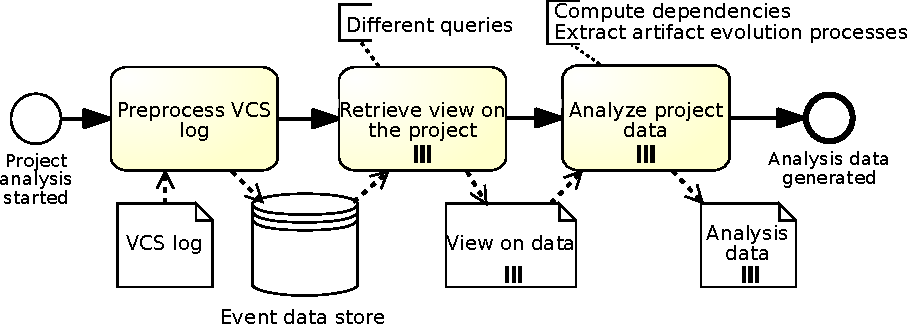
\includegraphics[width=.9\textwidth]{bpm2017/figures/visualization-process-crop}
	\caption[Approach for generating analysis data from VCS logs]{Approach for generating analysis data from VCS logs}
	\label{fig:visualization-process}
\end{figure}

The first step of the technique is the preprocessing of the \gls{vcs} log received as input. The main goal of this phase is to generate a set of events and store them into a database. Second, we obtain different views on the stored events. In particular, we are interested in observing
\begin{inparaenum}[\itshape i)]
	\item all the commits that affected the files over time;
	\item the amount of change brought by the commits to the files; and
	\item the users who issued such commits.
\end{inparaenum}
The third phase is responsible for considering the different perspectives defined by the project manager and through the generated views extract the necessary knowledge. In the following, we detail the formal concepts and the algorithm of our technique.



%We propose a techniques to extract and represent the work history and the dependencies among artifacts. The process is depicted in \Cref{fig:visualization-process} and consists of three successive steps towards extracting hidden work dependencies from \gls{vcs} event data. The method works under the following assumptions.

\begin{itemize}
\item [A1:] {\bf Meaningful file tree structure.} The file tree structure in a project represents the structure of work of the project participants.
\item [A2:] {\bf Frequent commits.} Commits to the VCS are regularly performed.  
\item [A3:] {\bf Meaningful comments.} The comments included by project participant when commiting their work represent the changes done to the file being commit.
\end{itemize}

\begin{figure}[h]
\centering
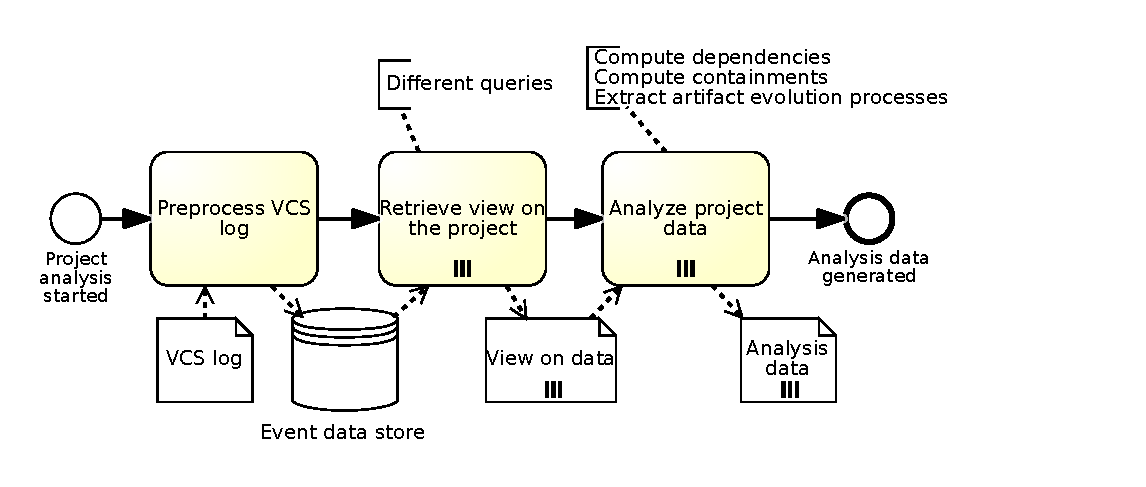
\includegraphics[width=.8\textwidth]{figures/visualization-process}
\caption[Generation of a process visualization from VCS logs]{Generation of a process visualization from VCS logs}
\label{fig:visualization-process}
\end{figure}

The first step of the approach is the preprocessing of the \gls{vcs} log received as input. The main goal of this phase is generate a set of events and store them into a database. Second, we obtain different views on the stored events. In particular, we are interested in observing
\begin{inparaenum}[\itshape i)]
	\item all the commits that affected the files over time;
	\item the amount of change brought by the commits to the files; and
	\item the users who issued such commits.
\end{inparaenum}
The third phase is responsible for considering the different perspectives defined by the project manager and through the generated views extract the necessary knowledge. The last phase is responsible for providing the visualization combining the different perspectives considered. In the following, we detail the formal concepts and the algorithm of our technique.

%\subsubsection{Preprocessing VCS Logs.}
%Version control system logs hold rich information about the artifacts and their evolution. Therefore, our process starts by extracting the elements \emph{Artifact}, \emph{Commit} and \emph{Event} from the log.
%
%First, the tree file is analyzed so the \emph{Parent} relation is defined. For that, the artifacts names appearing in the log are used. They provide the whole path from the root file until the leave file, which is the artifact in question. Thus, a parser can analyses the path and create the relation between the files. For instance, suppose we have the artifact \texttt{running example/software/model.java}. Three files are observed from this name: $f_1 = running \quad example$, $f_2 = software$ and $f_3 = model.java$. The following pairs will be included in the \emph{Parent} relation $\{(f_1,f_2),(f_2,f_3)\}$. 
%%are in the same containment if they share a common prefix that is maximal, i.e. they differ only by the name. For example, the files 
%%and \texttt{running example/software/test.java} . belong to the same containment, whereas the files  \texttt{running example/software/model.java} and \texttt{README.md} belong to two different containments. Note that containments can be contained in other containments, therefore every two files with eventually belong to the same containment. 
%
%Second, artifacts are extracted, as specified in Definition \ref{def_artifact}. Then the commits, following Definition \ref{def_commit}, are extracted. At last, the VCS raw log is transformed into a list of events for the extracted artifacts and commits, as specified in Definition \ref{def_event}. This step is easily done by replicating the information on commit level to be contained in the events. The amount of change is determined analyzing the attribute Diff of the VCS log. For instance, commit ID 2 in Table \ref{tab:vcs-log-data} indicates a commit with amount of change equals 3. The output of this phase is a set of events $E$, a set of artifacts $A$ and a set of commits $Com$.
%
%\subsubsection{Obtain View on Project.}
%The main goal of this phase is to extract the data that will be analyzed. The focus of this paper is in the artifacts, therefore the views generated gather information about events related to artifacts.  
%
%The project manager must determine the level of detail for the analyzes, thus, specifying the time windows. Input parameters of this phase are the interval of analysis ($ia$) and the time window for aggregation ($tw_{agg}$). Considering the specified $tw_{agg}$, the events generated in the previous phase are aggregated. For each artifact in a particular aggregate time an \emph{Aggregate Event} is generated as defined in Definition \ref{def_aggregateEvent}.
%
%\subsubsection{Analyze project data.}
%In this phase, the project is analyzed considering the different perspectives the project manager is interested in. In this paper, we considered three perspectives: dependency between artifacts, containments and artifact evolution.
%
%\paragraph{Dependency.} As stated in \Cref{def_dependency}, a dependency between two artifacts exists if both artifacts require a similar effort to be maintained, i.e. if they have a similar behavior considering the amount of changes.  The amount of change of an artifact over time defines  a time series. Therefore, for each artifact its aggregate events are analyzed in order to extract the amount of change for each aggregated time towards defining a time series for this artifact. 
%
%Let $AE$ be the set of aggregate events within $ia$. We build the time series for the \emph{i}-th artifact, namely $X_{f_i} = \lbrace (t, c) ~|~ e_a \in AE,~ t = ats(e_a),~ c = aac(e_a),~ f(e_a) = {f_i} \rbrace $. 
%
%%\todo[inline]{
%%Dependencies are obtained from the aggregated events. Considering the time window $tw$ and the aggregated event set in that time window ($AE_{tw}$), %$AE' = \lbrace e~|~ e \in AE,~ ts(e) \in tw \rbrace$,
%%we build the time series for the \emph{i}-th artifact, namely $X_{f_i} = \lbrace (t, c) ~|~ e_a \in AE_{tw},~ t = ats(e_a),~ t \in tw,~ c = aac(e_a),~ f(e_a) = {f_i} \rbrace $. As a result, the dependency between \emph{i}-th and the \emph{j}-th artifact is the correlation across time series $\sigma(i,j) = {corr(X_i, X_j)}$.
%%}
%
%After the time serie for each artifact is defined, the correlation function is used to calculate the correlation between the two time series. Considering artifacts $f_i$ and $f_j$ and the time series correspondent $X_{f_i}$ and $X_{f_j}$, $\sigma(f_i,f_j) = {corr(X_{f_i}, X_{f_j})}$ is the correlation value found when applying correlation function $corr$.
%
%If $\sigma(f_i,f_j)$ overcomes a threshold defined by the project manager (input parameter of this phase), then a dependency between the correspondent artifacts is established. The strength of the dependency is defined by $\sigma(f_i,f_j)$. 
%
%\paragraph{Containments.}
%For the containments extraction, the $Parent$ relation is analyzed and the set $C$ of containments defined.
%Containments reflect the hierarchical nature of the file structure in a repository. That is, \emph{composite containments} can be recursively decomposed into smaller containments until an \emph{atomic containment} is reached, following the tree structure of the file system top down. Conversely, from navigating the file structure bottom up, containments can be part of other containments until the root containment is reached. 
%
%
%\paragraph{Artifact evolution.}
%%For the artifact evolution definition, we propose to apply story mining techniques as follows.
%
%%\label{subsec:story-mining}

In a software development scenario, project participants add, remove, modify and perform several different operations in an artifact and store these changes in a shared repository (such as GitHub or Subversion). Different participants may change an artifact, and therefore it is a collaborative work towards a final product. Moreover, they can add comments when committing changes to an artifact bringing insights of the working process performed in this artifact.

We argue that these comments 
%form the textual elements is a kind of story being told, with additional elements such as location (the specific folder and files being manipulated at the broader view of a Project folder tree map) and the timestamp of their specific operation. The comments text and the additional elements
follow a similar structure of the story applied at the Story Mining method  \cite{Goncalves2011} , i.e., the comments provided by the different participants build the story about the work being done in the particular artifact. Moreover, additional elements such as time of the commit and the project participant responsible for the changes provide extra information that can be used to represent the artifact evolution. Therefore, in this research we use story mining to build a process which represents the artifact evolution. The input of the story mining is a set artifact stories, where the story of the \emph{i}-th artifact is obtained from the set $AE$ of aggregated events as $ story({f_i}) = \lbrace {m ~|~ a_e \in AE,~ f(a_e) = f_i,~ ak(a_e)=m} \rbrace$.


%several distinct visualizations from these stories to represent the software process elements, thus depicting critical viewpoints for the participants.
For instance, consider information about $4$ aggregate events related to a specific artifact as depicted in \Cref{table:ExampleOfComments}:

\begin{table}[!h]
	\caption{Comments made by project participants in four different times when committing changes performed in a artifact.}
	\label{table:ExampleOfComments}
\begin{center}
\begin{tabular}{|c|c|l|}
Time & Project Participant & Comment\\\hline
$ats_1$ & $au_1$ & Add requirements file. \\
$ats_2$ & $au_2$ &Update requirements.\\
$ats_3$ & $au_2$ &Modify requirements.\\
$ats_4$ & $au_2$ &Specify solved time for problem.\\
\end{tabular}
\end{center}
  
\end{table}

Using the story mining approach we are able to find the process activities. Then, considering the time of each commit, a workflow is created. Moreover, we associated the participant responsible for the work as the one that committed the changes. The final process discovered for the illustrative example is depicted in Figure \ref{fig:ExampleOfWorkingProcess}.

\begin{figure}[!h]
	\centering
  
\includegraphics[width=.9\linewidth]{ProcessExample}
  \caption{Working process generated from the set of comments depicted in Table
  \label{fig:ExampleOfWorkingProcess} \ref{table:ExampleOfComments}. The color images represent the user responsible for the commit.}
\end{figure}




 %\hfill\\
%1. Compute correlation - dependency
%2. Compute containments 
%3. Apply story mining to obtain the process  - artifact evolution \\\hfill

%\subsubsection{Generate visualization.}
%%The approach is flexible making possible to generate different visualizations 
%In this section, we define the graphical elements of the visualization and their semantic. 
%
%%\input{table/visual-symbols}
%\paragraph{Project Participant.}
%%\todo[inline]{Task was not defined before. I think in our case workload will be in how many changes the project participant is involved within a period of time. I change to this idea. See what do you think. \\[2pt] I also consider project participant instead of resource following what was defined in section II.A. But I am ok with both. We just need to decide and change the whole paper. \\[2pt] The symbols have different faces and the semantic was not provided. I know they align with the color, but I think it is better to have the same face (not all people with high workload are sad or with low workload are happy). On the other hand, we lost the representation of a participant in the process, i.e. we are not able to visualize how many different participant worked in the same process (artifact). If we are still interested in that, I suggest to leave the faces as symbolizing the workload and the colors to symbolize different participants}
%
%Project Participants are displayed through a face symbol with its identification in the top, as depicted in  \Cref{fig:resources}. We use a color code to denote their level of workload, i.e. in how many changes the project participant is involved in the project within $ia$. \emph{Red}, \emph{yellow} and \emph{green} color indicate \emph{high}, \emph{medium} and \emph{low} project workload respectively. The project workload for a project participant ($wl_u$) is computed from the set of events in which the project participant was responsible for the change within $ia$, i.e. $wl_u(t_1,t_2) = |\lbrace e \in E ~|~  u(e)= u, t_1 \leq ts(e) \leq t_2 \rbrace|$, where $ia=[t_1 , t_2]$. These interval of analysis can be fine tuned to visualize the project participant occupancy over time. 
%
%%\begin{figure}[h]
%%	\centering
%%	\begin{subfigure}{.3\linewidth}
%%		\centering
%%		\begin{tikzpicture}[scale=.2]
%%		\node[text width=3cm] at (2,2.3) {resource};
%%		
%%		\filldraw [color=black, fill=green!50] (0,0) circle (2);
%%		\filldraw [color=black, fill=white] (-0.5,.6) ellipse (0.2 and 0.6);
%%		\filldraw [color=black, fill=white] (0.5,.6) ellipse (0.2 and 0.6);
%%		\filldraw [color=black, fill=black] (-0.5,.4) ellipse (0.2 and 0.3);
%%		\filldraw [color=black, fill=black] (0.5,.4) ellipse (0.2 and 0.3);
%%		\draw  (-1,-0.5) .. controls (-0.5,-1) and (0.5,-1) .. (1,-0.5);
%%		\draw  (-1,-0.5) .. controls (-0.5,-1.3) and (0.5,-1.3) .. (1,-0.5);
%%		\fill[fill=white, draw=black, opacity=1] (-1,-0.5) .. controls (-0.5,-1) and (0.5,-1) .. (1,-0.5) .. controls (0.5,-1.3) and (-0.5,-1.3) .. (-1,-0.5) --cycle;
%%		\end{tikzpicture}
%%		%		
\includegraphics[width=.3\linewidth]{figures/visualization-elements/green-face}
%%		\caption{}
%%		\label{fig:green}
%%	\end{subfigure}%
%%	\begin{subfigure}{.3\linewidth}
%%		\centering
%%		%		
\includegraphics[width=.3\linewidth]{figures/visualization-elements/yellow-face}
%%		\begin{tikzpicture}[scale=.2]
%%		\filldraw [color=black, fill=yellow!50] (0,0) circle (2);
%%		\filldraw [color=black, fill=white] (-0.5,.6) ellipse (0.2 and 0.6);
%%		\filldraw [color=black, fill=white] (0.5,.6) ellipse (0.2 and 0.6);
%%		\filldraw [color=black, fill=black] (-0.5,.4) ellipse (0.2 and 0.3);
%%		\filldraw [color=black, fill=black] (0.5,.4) ellipse (0.2 and 0.3);
%%		%mouth
%%		%		\draw  (-1,-0.6) .. controls (-0.5,-1) and (0.5,-1) .. (1,-0.5);
%%		%	\draw  (-1,-0.5) .. controls (-0.5,-1.3) and (0.5,-1.3) .. (1,-0.5);
%%		\fill[fill=white, draw=black, opacity=1] (-1,-0.7) .. controls (-0.5,-0.8) and (0.5,-0.8) .. (1,-0.7) .. controls (0.5,-1) and (-0.5,-1) .. (-1,-0.7) --cycle;
%%		\end{tikzpicture}
%%		\caption{}
%%		\label{fig:yellow}
%%	\end{subfigure}%
%%	\begin{subfigure}{.3\linewidth}
%%		\centering
%%		%		
\includegraphics[width=.3\linewidth]{figures/visualization-elements/red-face}
%%		\begin{tikzpicture}[scale=.2]
%%		\filldraw [color=black, fill=red!60] (0,0) circle (2);
%%		\filldraw [color=black, fill=white] (-0.5,.6) ellipse (0.2 and 0.6);
%%		\filldraw [color=black, fill=white] (0.5,.6) ellipse (0.2 and 0.6);
%%		\filldraw [color=black, fill=black] (-0.5,.4) ellipse (0.2 and 0.3);
%%		\filldraw [color=black, fill=black] (0.5,.4) ellipse (0.2 and 0.3);
%%		%			\draw  (-1,-0.5) .. controls (-0.5,-1) and (0.5,-1) .. (1,-0.5);
%%		%		\draw  (-1,-0.5) .. controls (-0.5,-1.3) and (0.5,-1.3) .. (1,-0.5);
%%		\fill[fill=white, draw=black, opacity=1] (-1,-1) .. controls (-0.5,-0.5) and (0.5,-0.5) .. (1,-1) .. controls (0.5,-0.8) and (-0.5,-0.8) .. (-1,-1) --cycle;
%%		\end{tikzpicture}
%%		\caption{}
%%		\label{fig:red}
%%	\end{subfigure}
%%	\caption{Project Participant symbols. Color codes represent the status of their workload within a period of time.}
%%	\label{fig:resources}
%%\end{figure}
%
%
%%\begin{figure}[h]
%%	\centering
%%		\begin{tikzpicture}[scale=.2]
%%		\node[] at (0,3.5) {\textit{participant}};
%%		\filldraw [color=black, fill=white!50] (0,0) circle (2);
%%		\filldraw [color=black, fill=white] (-0.5,.6) ellipse (0.2 and 0.6);
%%		\filldraw [color=black, fill=white] (0.5,.6) ellipse (0.2 and 0.6);
%%		\filldraw [color=black, fill=black] (-0.5,.4) ellipse (0.2 and 0.3);
%%		\filldraw [color=black, fill=black] (0.5,.4) ellipse (0.2 and 0.3);
%%		%mouth
%%		%		\draw  (-1,-0.6) .. controls (-0.5,-1) and (0.5,-1) .. (1,-0.5);
%%		%	\draw  (-1,-0.5) .. controls (-0.5,-1.3) and (0.5,-1.3) .. (1,-0.5);
%%		\fill[fill=white, draw=black, opacity=1] (-1,-0.7) .. controls (-0.5,-0.8) and (0.5,-0.8) .. (1,-0.7) .. controls (0.5,-1) and (-0.5,-1) .. (-1,-0.7) --cycle;
%%		\end{tikzpicture}
%%	\caption{Project Participant symbol. The workload within a period of time is color coded.} 
%%	\label{fig:resources}
%%\end{figure}
%
%
%
%\paragraph{Dependency.}
%A dependency between two artifacts is represented by a line that connects their atomic containments. We label dependencies with a number  $\sigma \in \Re$, which indicates the strength of the dependency among the two artifacts. \Cref{fig:dependency} illustrate the notation for dependencies.
%
%%\begin{figure}[h]
%%	\centering
%%	%	
\includegraphics[width=0.7\linewidth]{figures/visualization-elements/dependency}
%%	\begin{tikzpicture}[scale=.5]
%%	\draw[thick] (-2,0) -- node[above,thick] {$\sigma$} ++(4,0);
%%	\end{tikzpicture}
%%	\caption{Dependency with strength $\sigma$}
%%	\label{fig:dependency}
%%\end{figure}
%
%\paragraph{Artifact evolution.}
%
%The artifact evolution is a process under which the artifact changes step by step towards a final state reached eventually in the project (e.g. a documentation file reaches his final state when the documentation is complete and no edits are made to that version of document anymore). Thus, we chose the \gls{bpmn} to represent this process. 
%
%\Cref{fig:process} depicts an example of a process learned considering a story with two aggregated comments, thus a process with two sequential activities \emph{a} and \emph{b}, modeled in \gls{bpmn}. 
%
%%\tikzstyle{startstop} = [rectangle, rounded corners, minimum width=1.5cm, minimum height=1cm,text centered, draw=black, fill=white!30]
%%\tikzstyle{arrow} = [thick,->,-latex]
%%\tikzstyle{event} = [circle,scale=.5, minimum width=1cm, minimum height=1cm,draw,fill=white]
%%\tikzstyle{end event} = [event,ultra thick]
%%
%%\begin{figure}[h]
%%	\centering
%%	%
\includegraphics[width=0.7\linewidth]{figures/visualization-elements/process}
%%	\begin{tikzpicture}[scale=.3]
%%	\begin{scope}[auto, every node/.style={draw,circle},node distance=.2cm]
%%	\node (start) [event] {};
%%	\node (add) [startstop, right of=start, xshift=1.3cm] {a};
%%	\node (fix) [startstop, right of=add, xshift=1.9cm] {b};
%%	\node (end) [end event, right of=fix, xshift=2.8cm] {};
%%	\draw [arrow]  (start) -- (add);
%%	\draw [arrow]  (add) -- (fix);
%%	\draw [arrow]  (fix) -- (end);
%%	\end{scope}
%%	\end{tikzpicture}
%%	\caption{Process representing an artifact evolution using \gls{bpmn}.}
%%	\label{fig:process}
%%\end{figure}
%
%
%\paragraph{Containment.} 
%A containment is represented with a rectangle. 
%We overload the semantic of rectangle used to represent the containment with a time concept. The position of the \emph{atomic containments} is shifted within the boundaries of their parent containments according to the first timestamp of the artifact history. For example, given two \emph{atomic containments} $C_1\{f_i\}$, $C_2\{f_j\} \subseteq C$, and let $AE_i, AE_j \subseteq AE$ be the sets of aggregated events that affected these artifacts, respectively. Then $C_1$ is shifted left with respect to $C_2$ if $min\{ats(e) | e \in AE_i\} < min\{ats(e') | e' \in AE_j\}$. \Cref{fig:containment} illustrates this example.
%
%%\begin{figure}[h]
%%\centering
%%%
\includegraphics[width=0.7\linewidth]{figures/visualization-elements/containment}
%%\usetikzlibrary{
%%	shapes.geometric,
%%	positioning,
%%	fit,
%%	calc
%%}
%%\begin{tikzpicture}
%%	\draw[thick] (0,0)rectangle (4,2) node[pos=.85] {$C_3$};
%%	\draw[thick] (1.1,1.1) rectangle (2.2,1.6) node[midway] {$C_1$}; 
%%	\draw[thick] (2.1,0.1) rectangle (3.2,0.6) node[midway] {$C_2$};
%%\end{tikzpicture}
%%\caption{A containment $C_3$ composed of two atomic containments $C_1$, $C_2$. $C_1$ is shifted more left wrt $C_2$ as its contained artifacts were affected by changes earlier.}
%%\label{fig:containment}
%%\end{figure}
%
%\begin{figure}
%	\centering
%	\begin{subfigure}[t]{.5\textwidth}
%		\centering
%		\begin{tikzpicture}[scale=.2]
%		\node[] at (0,3.5) {\textit{participant}};
%		\filldraw [color=black, fill=white!50] (0,0) circle (2);
%		\filldraw [color=black, fill=white] (-0.5,.6) ellipse (0.2 and 0.6);
%		\filldraw [color=black, fill=white] (0.5,.6) ellipse (0.2 and 0.6);
%		\filldraw [color=black, fill=black] (-0.5,.4) ellipse (0.2 and 0.3);
%		\filldraw [color=black, fill=black] (0.5,.4) ellipse (0.2 and 0.3);
%		%mouth
%		%		\draw  (-1,-0.6) .. controls (-0.5,-1) and (0.5,-1) .. (1,-0.5);
%		%	\draw  (-1,-0.5) .. controls (-0.5,-1.3) and (0.5,-1.3) .. (1,-0.5);
%		\fill[fill=white, draw=black, opacity=1] (-1,-0.7) .. controls (-0.5,-0.8) and (0.5,-0.8) .. (1,-0.7) .. controls (0.5,-1) and (-0.5,-1) .. (-1,-0.7) --cycle;
%		\end{tikzpicture}
%		\caption{Project Participant symbol. The workload within a period of time is color coded.} 
%		\label{fig:resources}
%	\end{subfigure}~
%	\begin{subfigure}[t]{.5\textwidth}
%		\centering
%		%	
\includegraphics[width=0.7\linewidth]{figures/visualization-elements/dependency}
%		\begin{tikzpicture}[scale=.5]
%		\draw[thick] (-2,0) -- node[above,thick] {$\sigma$} ++(4,0);
%		\end{tikzpicture}
%		\caption{Dependency with strength $\sigma$}
%		\label{fig:dependency}
%	\end{subfigure}\\
%	\begin{subfigure}[t]{.5\textwidth}
%		\tikzstyle{startstop} = [rectangle, rounded corners, minimum width=1.1cm, minimum height=.6cm,text centered, draw=black, fill=white!30]
%		\tikzstyle{arrow} = [thick,->,-latex]
%		\tikzstyle{event} = [circle,scale=.7, minimum width=.5cm, minimum height=.5cm,draw,fill=white]
%		\tikzstyle{end event} = [event,ultra thick]
%		%		\begin{figure}[h]
%		\centering
%		%
\includegraphics[width=0.7\linewidth]{figures/visualization-elements/process}
%		\begin{tikzpicture}
%		\begin{scope}[auto, every node/.style={draw,circle},node distance=.05cm]
%		\node (start) [event] {};
%		\node (add) [startstop, right of=start, xshift=1cm] {a};
%		\node (fix) [startstop, right of=add, xshift=1.5cm] {b};
%		\node (end) [end event, right of=fix, xshift=1.6cm] {};
%		\draw [arrow]  (start) -- (add);
%		\draw [arrow]  (add) -- (fix);
%		\draw [arrow]  (fix) -- (end);
%		\end{scope}
%		\end{tikzpicture}
%		\caption{Process representing an artifact evolution using \gls{bpmn}.}
%		\label{fig:process}
%		%		\end{figure}
%	\end{subfigure}~~
%	\begin{subfigure}[t]{.45\textwidth}
%		\centering
%		%
\includegraphics[width=0.7\linewidth]{figures/visualization-elements/containment}
%		\usetikzlibrary{
%			shapes.geometric,
%			positioning,
%			fit,
%			calc
%		}
%		\begin{tikzpicture}[scale=.99]
%		\draw[thick] (0,0)rectangle (4,2) node[pos=.85] {$C_3$};
%		\draw[thick] (1.1,1.1) rectangle (2.2,1.6) node[midway] {$C_1$}; 
%		\draw[thick] (2.1,0.1) rectangle (3.2,0.6) node[midway] {$C_2$};
%		\end{tikzpicture}
%		\caption{A containment $C_3$ composed of two atomic containments $C_1$, $C_2$. $C_1$ is shifted more left wrt $C_2$ as its contained artifacts were affected by changes earlier.}
%		\label{fig:containment}
%	\end{subfigure}
%	\caption{Graphic elements used to represent the defined concepts of project participant, work dependency, artifact evolution and containment.}
%\end{figure}
%
%\paragraph{Composing the visualization.}
%
%The layout rules to compose the visualization are the following. 
%\begin{inparaenum}[\itshape (i)]
%	\item Every element is within a containment, excluding the root;
%	\item Project participants responsible for the change are placed over \gls{bpmn} activities;
%	\item Artifact evolution is within an atomic containment;
%	\item Dependencies connect atomic containments, showing the strength of correlations between the belonging artifacts evolutions.
%\end{inparaenum}
%\Cref{fig:all-elements-together} shows the correct composition of the presented visual elements.
%
%\begin{figure}
%\centering
%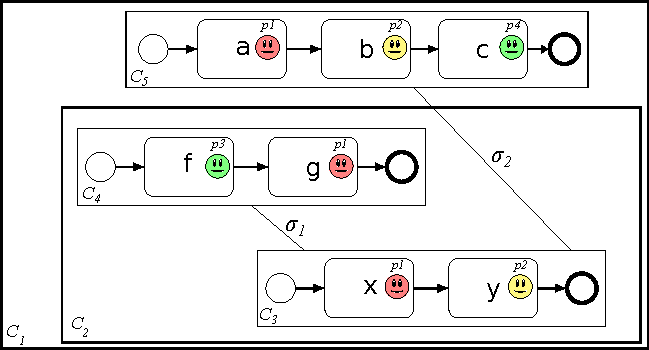
\includegraphics[width=.6\linewidth]{figures/visualization-elements/al-elements-together}
%\caption{Composition of the graphic elements into five containments, of which two are composite.}
%\label{fig:all-elements-together}
%\end{figure}



\subsection{Preliminaries}
\label{subsec:prelim}

%1. How we define/capture software processes\\

%2. How we define containment\\

%3. How we define dependencies\\

%Version control systems (VCSs) are used in projects to ensure reliable collaboration. We build our technique on \gls{vcs}. Typically, people work in VCS on files (e.g., text, source code, spread sheets) and commit them to the central repository. Project participants comment on their commits so that other participants can better understand the nature of the changes performed to the files.

As the objective of our technique is to uncover hidden work dependencies, we define the fundamental concepts required to capture them. Work is reflected by \emph{artifacts}, e.g., word documents, spreadsheets, code, etc. Artifacts are leaves in the file tree hierarchy (with directories being special type of non-leaf files). %Each directory in the file system groups together one or more files into a so-called \emph{containment}. 
Artifacts evolve over time, while project participants contribute their changes. Each change is an \emph{event} that happens to an artifact in a single point in time. Events can be abstracted into \emph{aggregated events} that allow a coarser grained view on the history. The history of the changes of an artifact over a time interval at a given level of abstraction is referred to as \emph{artifact evolution}. Similar artifact co-evolution establishes a \emph{dependency} between two artifacts. %In the following, we formally define the aforementioned concepts.

A software product is subdivided into files and directories. In this work, we consider directories as special type of files which are parents of other files. Formally, let $F$ be the universe of files in a software development project. Files are organized in a file tree. Therefore, each file $f \in F$ has one parent file. The only file without a parent file is the \emph{root} file. We capture this information in the parent relation $Parent: F \times F$. For example, let $f_p \in F$ be the parent of file $f_c \in F$, then $(f_p, f_c) \in Parent$. %Every file in $Parent$ defines a so-called \emph{containment}. For example, let $Parent = \{(f_{p_1} , f_{c_1})$, $(f_{p_1},f_{c_2})$, $(f_{p_2},f_{c_3})$, $(f_{p_3},f_{p_1})$,$(f_{p_3},f_{p_2})\}$, then files $f_{p_1}$, $f_{p_2}$ and $f_{p_3}$ define containments. Let $C$ be the set of containments. In our example $C=\{f_{p_1}, f_{p_2}, f_{p_3}\}$.
An \emph{artifact} is a file that is not a parent file, i.e. a file $f_a$ is an artifact if $\forall_{f \in F} (f_a, f) \notin Parent$.

%In this work, we are interested in describing the work progress related to a specific file, that we henceforth call \emph{artifact} and describe as follows:

%\begin{definition}
%	\label{def_artifact}
%	{\bf (Artifact)} An \emph{artifact} is a file that it is not a parent file, i.e. a file $f_a$ is an artifact if $\forall_{f \in F} (f_a, f) \notin Parent$.
%\end{definition}
%
%The files are grouped considering their organization in the tree file. We call each of these groups \emph{containments} and they are defined as follows:
%\begin{definition}
%\label{def_containment}
%{\bf (Containment)} A \emph{containment} is a file that is a parent of at least one other file. For example, let $Parent = \{(f_{p_1} , f_{c_1})$, $(f_{p_1},f_{c_2})$, $(f_{p_2},f_{c_3})$, $(f_{p_3},f_{p_1})$,$(f_{p_3},f_{p_2})\}$, then files $f_{p_1}$, $f_{p_2}$ and $f_{p_3}$ are containments. Let $C$ be the set of containments. In our example $C=\{f_{p_1}, f_{p_2}, f_{p_3}\}$.
%\end{definition}

%\begin{definition}
%	\label{def_artifact}
%	{\bf (File Containment)} An \emph{artifact} is a file that it is not a parent file, i.e. a file $f_a$ is an artifact if $\forall_{f \in F} (f_a, f) \notin Parent$.
%\end{definition}


%Containments can be either \emph{atomic} or \emph{composite}. An \emph{atomic containment} is a file which is parent of artifacts. In our example, containments $f_{p_1}$ and  $f_{p_2}$ are atomic containments.
%%\Cref{fig:containment} shows the visual symbol for an atomic containment.
%A \emph{composite containment} is a containment which is not atomic, i.e. it involves files which are parents of parents. In our example, containment $f_{p_3}$ is a \emph{composite containment}.  Therefore, the set $C$ of containments is partitioned in two subsets $C=C_1 \cup C_2$. In our example, $C=\{\{f_{p_1}, f_{p_2}\},\{f_{p_3}\}\}$.


% are defined, $C_1 = \{f_{c_1},f_{c_2}\}$ and $C_2=\{f_{c_3}\}$. A \emph{containment} $C$ is a set of files with the same parent file. For example, let $Parent = \{(f_{p_1} , f_{c_1}), (f_{p_1},f_{c_2}), (f_{p_2},f_{c_3})\}$, then two containments are defined, $C_1 = \{f_{c_1},f_{c_2}\}$ and $C_2=\{f_{c_3}\}$.

When project participants do a certain amount of work and want to save their current progress, they commit the changes to the \gls{vcs}. We define changes on artifacts as the \emph{events} of interest on the lowest granularity.

\begin{definition} {\bf(Event)}
\label{def_event}
Let $E$ be the set of events. An \emph{event} $e \in E$ is a five-tuple $(f, ac, ts, k,u)$, where
\begin{itemize}
\item $f \in F$ is the affected artifact of the event.
%\item $o \in O$ = \{added, modified, deleted\} is the change operation on the artifact with obvious meaning.
\item $ac \in AC =  \mathbb{N}$ is the amount of change done in the artifact.
\item $ts \in TS = \mathbb{N}$ represents a unix time stamp marking the time of the event occurrence.
\item $k \in \Sigma ^* $ is a comment in natural language text.
\item $u \in U$ is the project participant responsible for the change.
\end{itemize}
\end{definition}

For event $e = (f, ac, ts, k,u)$ we overload $f$, $ac$, $ts$, $k$ and $u$ to be used as accessor functions. For example, $f$ is the function $f : E \rightarrow F$ mapping an event to its affected artifact.

In some situations, it can be interesting to have a higher level overview of the changes done to a particular artifact. In this case, an aggregation of events related to this artifact in an interval of time can be performed. The time window for the aggregation, henceforth denoted as $tw_{agg}$, must be defined, i.e. the size of the time interval. For instance, a time window for aggregation can be a day. Thus, all events occurring for an artifact in the same day will be aggregated. An \emph{aggregated event} is defined as follows:

\begin{definition} {\bf (Aggregated Event)}
\label{def_aggregateEvent}
An \emph{Aggregated Event} for $tw_{agg}$ ($AE_{tw_{agg}}$) is a five-tuple $(f, aac, ats, ak,au)$, where
\begin{itemize}
\item $f \in F$ is the affected artifact in the set of events being aggregated.
%\item $ao \in O$ = \{added, modified, deleted\} is the aggregated change operation on the artifact. If the only change operation performed in $tw_{agg}$ was \emph{added} or \emph{deleted} then the aggregated change operation is the same, otherwise it is \emph{modified}.
\item $aac \in AAC =  \mathbb{N}$ is the aggregate amount of change done in the artifact for $tw_{agg}$. It is calculated by summing the amount of changes done in each of the time aggregated.
\item $ats \in ATS = \mathbb{N}$ represents an aggregate time of the unix time stamp of the events being aggregated.
\item $ak \in \Sigma ^* $ is the concatenation of the comments presented in the events being aggregated.
\item $au \subseteq U$ are the project participants responsible for the changes in $tw_{agg}$ being aggregated.
\end{itemize}
\end{definition}
%\todo[inline]{We consider a $tw$ but do not use it in the definition.}

The set of aggregated events for a particular artifact defines how this artifact evolves over time. Considering an interval of analysis, henceforth denoted as $ia$, we define artifact evolution as follows.

\begin{definition} {\bf (Artifact Evolution)}
%Let $EA_f$ be the set of all aggregated events related to artifact $f$.
\emph{Artifact evolution} is the process describing how the file $f$ changed over an interval of time $ia$, i.e., a set of labeled tuples $A_{evo}(f) = \{ (t,a,l) | e \in AE_{ia}, f=f(e), t=ats(e), a=aac, l=ak(e)\}$ chronologically ordered.

%The comments associated to the aggregated events in $EA_f$ define the activities executed. The time of the aggregated events in $EA_f$ establishes the order of the activities and then the flow of evolution. Each activity is associated with the user that executed it.
\end{definition}

%Project participants can commit a number of changes to different artifacts at one step. Therefore, we define the notion of commits as follows.
%
%\begin{definition} {\bf (Commit)}
%\label{def_commit}
%A \emph{commit} $Com$ is a set of events sharing the same time stamp and comment, i.e., $\forall e, e'\in Com : ts(e) = ts(e')\wedge k(e) = k(e')$. Additionally, each event in a commit affects different artifact, i.e., $\forall e, e' \in Com : e \neq e' \rightarrow f(e) \neq f(e')$.
%\end{definition}

%For example, a dependency is established if the two artifacts require a similar effort to be maintained. The effort of maintenance is measured through the amount of changes done to the artifact.

%\begin{definition} {\bf (Dependency)}
%\label{def_dependency}
%A \emph{dependency} between two artifacts within $ia$ is a similarity function $\sigma : X_{evo} \times X_{evo} \rightarrow \mathbb{Z}$, where the artifact evolution set in which the labels are projected out, i.e $X_{evo} = \{(t,a) | \exists l : (t,a,l) \in A_{evo}\}$.
%%Thus, each artifact defines a time series of the amount of change. If the correlation between two time series is significant then a dependency between the correspondent artifacts is established. The strength of the dependency is defined by the correlation value.
%\end{definition}
%
%
%
%\subsection{Metrics} 

Note that artifact evolution represents the changes that happened to a file over time. Thus, we can build the time series of a file $f$ as the vectors of changes $\vec{X_{f}} = (a_1, ..., a_n)$ in the time window $tw_{agg} = [t_1,t_n]$, with $a_i$ being the sum of the changes of $f$ in of the aggregated intervals $t_i$ of the time window $tw_{agg}$.

%The file system establishes a structural tree-based relationship among files. However, other types of dependencies can emerge between two files. In this paper, we define dependency between two files in terms of their \emph{degree of co-evolution}.
%In this paper, we are interested in measuring the hidden work-dependencies among artifacts of the project-oriented business process. That is, we want to capture dependencies that are created among files that go beyond functional (e.g. interface-implementing class) or structural (e.g., parent-child in the file tree structure).

%We define the metrics of \emph{degree of co-evolution} and \emph{file distance}. 

We measure the dependency between two files $f_a$ and $f_b$ in terms of their \emph{degree of co-evolution} as follows.
\begin{definition} {\bf (Degree of Co-Evolution)} 
	\label{definition:degree-of-coevolution}
	Given two files $f_a$ and $f_b$, the \emph{degree of co-evolution} $\chi: F \times F \rightarrow [0,1]$ is a similarity function of the respective time series.
\end{definition}
In this paper, we fix $\chi(f_a,f_b) = |\sigma (\vec{X_{f_a}}, \vec{X_{f_b}})|$, where $\sigma$ is the correlation function of the two vectors $\vec{X_{f_a}}$ and $ \vec{X_{f_b}}$.

The way files are kept in the directory structure establishes an inherent relationship among files being stored close to each other in the hierarchy. For instance, files serving the same purpose are stored close to each other in the file system. 
Hidden work dependencies are expected to happen between artifacts that are distant in the file structure. We measure this distance as the length of the shortest route connecting two files in the file tree. We adapt the notion of path from~\cite{Gubichev2010} to our file tree. Given a file $f$, the path to the root node can be obtained by navigating the $Parent$ relationship up to the root file. The path $p$ from $f_a$ to the root $f_r$ is the set of parent files encountered along such route. i.e. $p(f_1,f_{r}) = \{(f_1, ..., f_k, f_{k+1}, ..., f_{r})\}$ such that for any $k$, $(f_{k+1},f_k) \in Parent $. The length of the path is the cardinality $|p|$ of the set. 
The shortest path between two files $f_a$, $f_b$ in a tree passes through the \gls{lca}~\citep{Bender2000}. This is equivalent to considering the paths from the single files to the root node $p_a = p(f_a,f_r)$ and $p_b=p(f_b, f_r)$ minus their intersection $I_{p_a,p_b}=\{p(f_a, f_r) \cap p(f_b, f_r)\}$. Thus, we define the \emph{file distance} as the length of the shortest path between two files $f_a$ and $f_b$ as follows. 

\begin{definition} {\bf (File Distance)} 
	\label{definition:artifact-distance}
	The distance $d : F \times F \rightarrow \mathbb{N} $ between two files belonging to the same directory structure is defined as the number of nodes in the minimum path connecting the two files in the project file tree: $d(f_a,f_b) =  |p_a| + |p_b| - 2*(|I_{p_a,p_b}|)$.
\end{definition}
 

\subsection{Hidden Dependencies Discovery Algorithm}

We are focused on finding interesting hidden work dependencies. These dependencies are typically reflected by changes that happen to couples of allegedly unrelated files during their evolution. This section details the procedure that implements the technique outlined in \Cref{fig:visualization-process}.

\Cref{algorithm:all} presents the steps required to explicate such hidden dependencies. The procedure $\mathtt{PreprocessLog(\mathcal{L})}$ in line~\ref{step:preprocess} takes as input a VCS log $\mathcal{L}$ structured as in \Cref{tab:vcs-log-data} and parses out work events at the granularity of line changes. These events are then stored into an event data storage. Events parsed from \gls{vcs} logs contain rich information about multiple aspects of the work they reflect. In order to represent all these different aspects, we devised the entity-relationship data model. Hence, we are able to store all the information that is possible to obtain after parsing the \gls{vcs} log. Furthermore, this step allows the user to obtain simple information, such as statistics on the project, already at an early stage of the procedure. The output of the $\mathtt{PreprocessLog(\mathcal{L})}$ step results in the storage of all the events $E$ into a database.
%Further on, we will show a possible implementation that uses a database to store the parsed events, but in principle any type of repository that allows to store the preprocessed events can be considered.

%\begin{figure}
%	\centering
%	\includegraphics[width=.8\textwidth]{figures/CommitLogER3.pdf}
%	\caption{Entity-Relationship model used to store events extracted from VCS logs}
%	\label{fig:data-model}
%\end{figure}


Next, the iterative call of the procedure $\mathtt{RetrieveView(\mathit{E}, \mathsf{query})}$ in line \ref{step:retrieve-view} performs several querying the data storage containing the set $E$. For example, a possible query can obtain all the comments associated to each change of a specific file. To obtain information on the evolution of files, we query the database for the changes of all the files within a user defined time interval $tw_{agg}$. In general several time frames can be chosen, each of them producing a \emph{view} $V$ on the data, i.e., a set of aggregated events chronologically sorted within $tw_{agg}$. For example, users may be interested in artifact-views aggregated by day, by month, etc. Multiple \emph{views} are possible by defining them in the {\textsf{queries}} parameter. We collect these views into a set $\mathcal{V} = \bigcup_{\textsf{queries}} V$. 

%Step~\ref{step:contaiments} extracts the structural relationships among the file paths contained in each view $V$, i.e., it recreates the file tree from the artifacts.


%\IncMargin{-1em}
%\setlength{\textfloatsep}{0pt}% Remove \textfloatsep
\begin{algorithm}
\SetKwData{Left}{left}\SetKwData{This}{this}\SetKwData{Up}{up}
\SetKwData{Views}{desiredviews}
\SetKwData{ViewType}{queries}
\SetKwFunction{PreprocessLog}{PreprocessLog}
\SetKwFunction{RetrieveView}{RetrieveView}
\SetKwFunction{ComputeDependencies}{ComputeDependencies}
\SetKwFunction{ComputeContainments}{ComputeContainments}
\SetKwFunction{ComputeEvolution}{ComputeEvolution}
\SetKwFunction{StoryMining}{StoryMining}

\SetKwInOut{Input}{Input}\SetKwInOut{Output}{Output}
\SetKwInOut{Data}{Data} \SetKwInOut{Data}{Data}
\Input{A VCS log $\mathcal{L}$}
\Output{A set of triples $\{(Dist,Stories,D_{co-evo})\}$, artifact evolutions, and dependencies}
\Data{$E$ event set, $\mathcal{V}$ views set, $AnalysisData = \{(Dist,Stories,D_{co-evo})\}$, degree of co-evolution threshold $\gamma$, file distance threshold $\delta$, user defined queries \ViewType }
\BlankLine
$Files \leftarrow \emptyset $, $Stories \leftarrow \emptyset$, $TimeSeries \leftarrow \emptyset$, $AnalysisData \leftarrow \emptyset$, $\mathcal{V} \leftarrow \emptyset$, $A_{evo}(f) \leftarrow \emptyset$\;
\tcc{Preprocess VCS log}
$E \leftarrow $ \PreprocessLog{$\mathcal{L}$}\;\label{step:preprocess}
\tcc{Retrieve views on the project}
\lFor{$i$ from $1$ \KwTo $|\ViewType|$}{
	$\mathcal{V} \leftarrow \mathcal{V} ~\cup $ \RetrieveView{$E$, $\ViewType\mathit{[i]}$}}\label{step:retrieve-view}
\tcc{Analyze project data}
%$C \leftarrow$ \ComputeContainments{$\mathcal{V}$}\; \label{step:contaiments}
%$A_{evo} \leftarrow $ \ComputeEvolution{$\mathcal{V}$}\; \label{step:evolution}
\ForEach{view $V \in \mathcal{V}$}{\label{step:evolution}
	\ForEach{aggreagated event $ae \in V$}{\label{step:forall-ae}
		\ForEach{$f=f(ae), t = ats(ae), a=aac(ae), l=aak(ae) \in ae$}{
			\tcc{Construct the artifact evolution set for the file}
			$A_{evo}(f) \leftarrow A_{evo}(f) \cup \{(t,a,l)\}$\;\label{step:a-evo}
			\tcc{Construct the process using story mining}
			$Stories \leftarrow Stories ~\cup (f,$ \StoryMining{$l$}$)$)\;\label{step:story-mining}
			\tcc{Collect files and time series}
			$Files \leftarrow Files \cup \{f\}$\;
			$TimeSeries(f) \leftarrow$ construct time series from $A_{evo}(f)$\; \label{step:timeseries}
		}
	}\label{step:forall-ae-end}
	\ForEach{pair of files $i, j \in Files$}{\label{step:metric-start}
		\tcc{Compute degree of co-evolution}\label{step:dependencies}
		$coEvoDegree \leftarrow \chi(TimesSeries(i), TimeSeries(j)) $\;
		\tcc{Compute file distances}\label{step:distances}
		$distance \leftarrow d(i,j)$\;
		\tcc{Select based on user defined thresholds}
		\lIf{$coEvoDegree > \gamma$}{$D_{co-evo} \leftarrow D_{co-evo} \cup \{coEvoDegree\}$}\label{step:threshold-co-evo}
		\lIf{$distance > \delta$}{$Dist \leftarrow Dist \cup \{distance\}$}\label{step:threshold-co-dist}
	}\label{step:metric-end}
	$AnalysisData \leftarrow AnalysisData \cup \{Dist,Stories,D_{co-evo}\}$\;\label{step:analysis-data}
}
\Return $AnalysisData$\;\label{step:analysis-data-return}
\caption{Generate project analysis data}
\label{algorithm:all}
\end{algorithm}%\DecMargin{1em}

%
%
%\For{$i\leftarrow 2$ \KwTo $l$}{
%\emph{special treatment of the first element of line $i$}\;
%\For{$j\leftarrow 2$ \KwTo $w$}{\label{forins}
%\Left$\leftarrow$ \FindCompress{$Im[i,j-1]$}\;
%\Up$\leftarrow$ \FindCompress{$Im[i-1,]$}\;
%\This$\leftarrow$ \FindCompress{$Im[i,j]$}\;
%\If(\tcp*[h]{O(\Left,\This)==1}){\Left compatible with \This}{\label{lt}
%\lIf{\Left $<$ \This}{\Union{\Left,\This}}
%\lElse{\Union{\This,\Left}}
%}
%\If(\tcp*[f]{O(\Up,\This)==1}){\Up compatible with \This}{\label{ut}
%\lIf{\Up $<$ \This}{\Union{\Up,\This}}
%\tcp{\This is put under \Up to keep tree as flat as possible}\label{cmt}
%\lElse{\Union{\This,\Up}}\tcp*[h]{\This linked to \Up}\label{lelse}
%}
%}
%\lForEach{element $e$ of the line $i$}{\FindCompress{p}}
%}
%%\IncMargin{1em}
\begin{algorithm}[H]
	\SetKwData{Left}{left}\SetKwData{This}{this}\SetKwData{Up}{up}
	\SetKwData{Views}{desiredviews}
	\SetKwFunction{PreprocessLog}{PreprocessLog}
	\SetKwFunction{RetrieveView}{RetrieveView}
	\SetKwFunction{ComputeDependencies}{ComputeDependencies}
	\SetKwFunction{ComputeContainments}{ComputeContainments}
	\SetKwFunction{ComputeEvolution}{ComputeEvolution}
	
	\SetKwInOut{Input}{Input}\SetKwInOut{Output}{Output}
	\SetKwInOut{Data}{Data}
	\Input{A VCS log $\mathcal{L}$}
	\Output{A set of triples $\{(C,A_{evo},D)\}$, respectively containments, artifact evolutions, and dependencies}
	\Data{$E$ event set, $V$ views set, $AD = \{(C,A_{evo},D)\}$ }
	\BlankLine
	
	$E \leftarrow $ \PreprocessLog{$\mathcal{L}$}\;
	\For{$i\leftarrow 1$ \KwTo \Views}{
		$V \leftarrow V \cup $ \RetrieveView{$E$}\;
	}
	$C \leftarrow$ \ComputeContainments{$V$}\;
	$D \leftarrow $ \ComputeDependencies{$V$}\;
	$A_{evo} \leftarrow $ \ComputeEvolution{$V$}\;
	$AD \leftarrow (C,A_{evo},D)$
	\caption{Retrieve view on data}
	\label{algorithm:retrieve-view}
\end{algorithm}
%\Cref{algorithm:compute-containments} computes the containments. Note that both atomic and composite containments are computed.

%%\IncMargin{1em}
\begin{algorithm}[H]
\SetKwData{Left}{left}\SetKwData{This}{this}\SetKwData{Up}{up}
\SetKwData{Views}{desiredviews}
\SetKwData{ViewType}{query}
\SetKwFunction{PreprocessLog}{PreprocessLog}
\SetKwFunction{RetrieveView}{RetrieveView}
\SetKwFunction{ComputeDependencies}{ComputeDependencies}
\SetKwFunction{ComputeContainments}{ComputeContainments}
\SetKwFunction{ComputeEvolution}{ComputeEvolution}

\SetKwInOut{Input}{Input}\SetKwInOut{Output}{Output}
\SetKwInOut{Data}{Data}
\Input{A set of views $\mathcal{V}$}
\Output{A set of containments $C$}
%\Data{$E$ event set, $\mathcal{V}$ views set, $Parent$ }
\BlankLine
$Parent \leftarrow \{(\emptyset, \emptyset)\} $, $C \leftarrow \emptyset$\;
\ForAll{$V \in \mathcal{V}$}{
	\lForEach{$f \in getFiles(V) $}{
		$Parent \leftarrow Parent \cup getParents(f)$}
}

\ForEach{$(f_p,f_{c_1}) \in Parent$}{
	\ForEach{$(f_p,f_{c_2}) \in Parent$}{
		\lIf{$f_{c_1} \neq f_{c_2} $}{$C \leftarrow C \cup \{f_{p}\}$}   
	}
}
\Return $C$\;
\caption{Compute artifact containments}
\label{algorithm:compute-containments}
\end{algorithm}

The step in line~\ref{step:evolution} starts an iteration over the views set $\mathcal{V}$. Here is where we collect the analysis data that are returned by the algorithm. For each of the aggregated artifacts contained in a view $V$, we retrieve the information necessary to compute the \emph{degree of co-evolution} between pairs of files and their \emph{file distance}. First, we construct the artifact evolution of all the artifacts present in $ae \in V$. 
Note that an aggregated event $ae \in V$ is a record obtained from a view on the project which is composed, among other attributes (e.g., file, time, amount of change), by the comment associated to the specific change. Comments describe multiple changes executed on the file, i.e. they describe a \emph{story} of the artifact. 
Stories associated to each file are collected and the corresponding labels are chronologically ordered. These file stories are then input to the StoryMining technique~\citep{Goncalves2011}. Story Mining was designed to receive as input a story freely written by the participants, describing their work in a particular business process. As an output, the \emph{actors} and the process \emph{activities} executed by them are extracted. Our technique is concerned with the stories of the files. Therefore, they are the actors of the story mining, and the resulting business process consists of the steps describing their evolution process. We collect the resulting processes in the step in line~\ref{step:story-mining}.
The step in line~\ref{step:timeseries} is concerned with the construction of a time series from the set of artifact evolutions $A_{evo}$ computed in line~\ref{step:a-evo}. Specifically, this step gathers the values of the changes of each of the artifact $f$ in $A_{evo}$ and records them in $TimeSeries(f)$. 

After all the aggregated events $ae$ have been explored, the algorithm moves on to computing the metrics (lines~\ref{step:metric-start}--\ref{step:metric-end}). In this loop, the algorithm iterates through all the pairs of files. For each pair, the \emph{degree of co-evolution} and \emph{artifact-distance}  metrics are computed according the \Cref{definition:degree-of-coevolution} and \Cref{definition:artifact-distance}, respectively. These two measures are collected only if their values are above the user defined thresholds $\gamma$ and $\delta$. After the loop is over, the two measurements and the stories mined with the StoryMiner are stored in $AnalysisData$.

Finally, after iterating over all the user defined views, the algorithm returns the $AnalysisData$ collection which can now be further inspected and analyzed in more detail, as we show next with an example.

%%\IncMargin{1em}
\setlength{\textfloatsep}{0pt}% Remove \textfloatsep
\begin{algorithm}[H]
\SetKwData{Changes}{changeAmount}\SetKwData{This}{this}\SetKwData{Up}{up}
\SetKwData{Time}{time}
\SetKwData{Labels}{labels}
\SetKwData{Stories}{Stories}
\SetKwFunction{StoryMining}{StoryMining}

\SetKwInOut{Input}{Input}\SetKwInOut{Output}{Output}

\Input{A set $\mathcal{V}$ of views}
\Output{A set of processes $A_{evo}$, A file stories collection $Stories$}
%\Data{$E$ event set, $\mathcal{V}$ views set, $Parent$ }
\BlankLine
$A_{evo} \leftarrow \emptyset$, $Stories \leftarrow \emptyset$\; 
\ForEach{$V \in \mathcal{V}$}{
	\ForEach{$ae \in V$}{
		$f \leftarrow getFile(ae)$\;
		$t \leftarrow getTime(ae)$\;
		$c \leftarrow getChangeAmount(ae)$\;
		$Labels \leftarrow getComments(ae)$\;
		$S \leftarrow S \cup (f, Labels) $\;
		\lForEach{$l \in Label$}{
			$A_{evo} \leftarrow A_{evo} \cup \{(t,c,l)\}$}
	}
	\lForEach{$(f,l) \in S$}{		
		$Stories \leftarrow Stories ~\cup (f,$ \StoryMining{$l$}$)$)}
}
\caption{Compute artifact evolution}
\label{algorithm:compute-evolution}
\end{algorithm}



%%\IncMargin{1em}
\setlength{\textfloatsep}{0pt}% Remove \textfloatsep
\begin{algorithm}[H]
\SetKwData{Left}{left}\SetKwData{This}{this}\SetKwData{Up}{up}
\SetKwData{Views}{desiredviews}
\SetKwData{ViewType}{query}
\SetKwFunction{PreprocessLog}{PreprocessLog}
\SetKwFunction{RetrieveView}{RetrieveView}
\SetKwFunction{ComputeDependencies}{ComputeDependencies}
\SetKwFunction{ComputeContainments}{ComputeContainments}
\SetKwFunction{ComputeEvolution}{ComputeEvolution}

\SetKwInOut{Input}{Input}\SetKwInOut{Output}{Output}
\SetKwInOut{Data}{Data}
\Input{A set of views $\mathcal{V}$, a similarity function $\sigma$, a filter parameter $\delta$}
\Output{A set of dependencies $D$}
%\Data{$E$ event set, $V$ views set, $AD = \{(C,A_{evo},D)\}$ }
\BlankLine

$X_f \leftarrow \emptyset$, $D \leftarrow \emptyset$\;
\ForEach{$V \in \mathcal{V}$}{
	\ForEach{$ae \in V$}{
		$t \leftarrow getTime(ae)$\;
		$c \leftarrow getChangeAmount(ae)$\;
		$f_i \leftarrow getFile(ae)$\;
		$X_{f_i} \leftarrow \{(t,c)\} \cup X_{f_i}$\;
	}
	$X_f \leftarrow X_f \cup \{X_{f_i}\}$\;
}

\ForEach{$i, j \in range(1:|X_f|) \wedge i \neq j $}{ \label{algo:comparison}
	$X_{f_i} \leftarrow get(X_f, i)$, $X_{f_j} \leftarrow get(X_f, j)$\;
	$T \leftarrow \{getTimes(X_{f_i})\} \cup \{getTimes(X_{f_j})\} $\;
	\ForEach{$t \in T$}{
		\lIf{$t \notin getTimes(X_{f_i}) $}{
			$X_{f_i} \leftarrow X_{f_i} \cup \{(t,0)\}$}
		\lIf{$t \notin getTimes(X_{f_j}) $}{
			$X_{f_j} \leftarrow X_{f_j} \cup \{(t,0)\}$}
	}
	\lIf{$|\sigma(X_{f_i}, X_{f_j})| > \delta $}{
		$D \leftarrow D \cup \{{(X_{f_i}, X_{f_j}, \sigma(X_{f_i}, X_{f_j}}))\} $}
}

\caption{Compute dependencies}
\label{algorithm:compute-dependencies}
\end{algorithm}
%
%The algorithm iterates over the views and creates the time series from the aggregated events $v$ in each of the views $V$ of the view collections $\mathcal{V}$. A time series is captured by a set $X_{f_i}$, recording the trend of the changes of file $f_i$ over the time. Next, the dependencies are calculated by using the similarity function $\sigma$ (cf. \Cref{def_dependency}) pairwise over the time series of the different artifacts. We do not enforce a determined similarity function between time series. The user can adopt a customized time series similarity function or use an existing method from literature (e.g.~\cite{ruohonen2015time}). Because the time series must have equal length, we add missing times $t$ with couples $(t,0)$. These couples denote that the amount of change in $f$ at time $t$ was 0. Finally, we collect the results in the dependencies set $D$ if they are stronger than the threshold $\delta$.



%\subsection{Metrics}

We are interested in measuring the hidden work dependencies among artifacts of the project-oriented business process. Therefore we define the metrics of \emph{degree of co-evolution} and \emph{file distance}. The degree of co-evolution is used to indicate dependency relations between files. We focus on the similarity of the evolution between two files $f_a$ and $f_b$. We build the time series for each of the files as the vectors of changes over time $\vec{X_{f_a}} = (c_1^a, ..., c_n^a)$ and $\vec{X_{f_b}} = (c_1^b, ..., ,c_n^b)$, where the indexes of $i \in [1,n]$ are of the corresponding aggregated time event in the time windows $tw_{agg} = [t_1,t_n]$, and $c_i^j$ are the changes in the aggregated period $t_i$ of the file $f_j$. We measure the co-evolution of two artifacts as the absolute value of the correlation $\sigma(f_a,f_b)$ of the respective time series.

\begin{definition} {\bf (Degree of Co-Evolution)} 
	\label{definition:degree-of-coevolution}
	The \emph{degree of co-evolution} is a function $\chi: F \times F \rightarrow [0,1]$. 
	\[
	\chi(f_a,f_b) = |\sigma (\vec{X_{f_a}}, \vec{X_{f_b}})|
	\]	
\end{definition}


Hidden work dependencies lie between artifacts that are distant in the file structure. We measure this distance as the length of the shortest route connecting two files in the file tree. We adapt the notion of path from~\cite{Gubichev2010} to our file tree. Given a file $f$ the path to the root node can be obtained by navigating the $Parent$ relationship up to the root file. The path $p$ from $f_a$ to the root $f_r$ is the set of parent files encountered along such route. i.e. $p(f_1,f_{r}) = \{(f_1, ..., f_k, f_{k+1}, ..., f_{r})\}$ such that for any $k$, $(f_{k+1},f_k) \in Parent $. The length of the path is the cardinality $|p|$ of the set.
The shortest path between two files $f_a$, $f_b$ in a tree passes through the \gls{lca}~\cite{Bender2000}. This is equivalent to considering the paths from the single files to the root node $p_a = p(f_a,f_r)$ and $p_b=p(f_b, f_r)$ minus their intersection $I_{p_a,p_b}=\{p(f_a, f_r) \cap p(f_b, f_r)\}$. Thus, we define the artifact distance as the length of the shortest path between two files $f_a$ and $f_b$ as follows.

\begin{definition} {\bf (File Distance)} 
	The distance $d : F \times F \rightarrow \mathbf{N} $ between two artifacts is defined as the number of steps in minimum path connecting the two artifacts in the file tree.
	\label{definition:artifact-distance}
	\[
	d(f_a,f_b) = 
	\begin{cases}
	
	1 + |p_a| + |p_b| - 2*(|I_{p_a,p_b}|) & \text{if $(I_{p_a,p_b}) \neq \emptyset $} \\
	0 & \text{otherwise}
	
	\end{cases}
	\]	
\end{definition}

%, i.e. two artifacts that belong to the same containment have distance 0, and the maximum distance possible between two artifacts is equal to twice the tree depth.



%\subsection{Story Mining}
\label{subsec:story-mining}

%What is story mining and how we use it in our work
Gon\c{c}alves et al.~\cite{Goncalves2011} proposed a story mining approach to extract process elements from stories, i.e. text descriptions written collaboratively by the process participants. A story is a natural way to transmit and share knowledge. Using both natural language (text) and contextual elements (categorization of parts of the story), storytellers can express their experience and viewpoints about the work processes they participate, interact with and/or perceive. Stories have the advantage of reproducing the situations associated with their contexts - the knowledge that is difficult to capture in interviews or mining from Information Systems logs. Since collectively told, a story incorporates a range of perspectives. Business processes instances can also be viewed as stories played by individuals who perform specific roles depending on the circumstances.

Story Mining  \cite{Goncalves2011} receives as input a story freely written by the participants, describing their work in a particular business process. As an output, the \emph{actors} and the process \emph{activities} executed by them are extracted. To illustrate the approach consider the following story. The terms highlighted in {\bf bold} are the actors of the processes and the terms highlighted in {\color{gray} gray} the activities. 

\begin{figure}[!h]
{ \bf The system} {\color{gray} generates an estimating template consisting of the phases, activities and tasks} selected
for the project or project phase. When planning complete projects the estimating is typically done at the activity level, using the
list of tasks in the work breakdown as input to the estimating process. However {\bf estimators} will likely {\color{gray}add an itemized list of system functions and other deliverables}, to facilitate estimating the construction phase. {\bf Multiple estimators} {\color{gray} prepare estimates for each component}, {\color{gray}compare their estimates}, and {\color{gray}arrive at a final estimate} for each item.
  \label{RB}
\end{figure}

A further step that we developed in our approach is the identification of the relationship between the activities, therefore defining the flow.

%\subsection{Project Mining Software Projects}
\label{subsec:proj-mining}

Project mining technique 

